\documentclass[11pt]{article}

\newcommand{\team}{\textit{Professor Chandrakesan}}
\newcommand{\ps}{SuperUROP Proposal}

%\pagestyle{headings}
\usepackage{amsfonts}
\usepackage{amssymb}
\usepackage{amsmath}
\usepackage{latexsym}
\usepackage{enumitem}
\usepackage{graphicx}
\usepackage{url}
\setlength{\parskip}{1pc}
\setlength{\parindent}{0pt}
\setlength{\topmargin}{-3pc}
\setlength{\textheight}{9.5in}
\setlength{\oddsidemargin}{0pc}
\setlength{\evensidemargin}{0pc}
\setlength{\textwidth}{6.5in}

\newcommand{\answer}[1]{
\newpage
\noindent
\framebox{
	\vbox{
		Skanda Koppula \hfill {\bf \ps} \hfill #1  \\ 
		\team \hfill \today
	}
}
\bigskip

}


\begin{document}
\answer{Digital Circuits Group}
This project focuses on the development of two separate but related, end-to-end secure systems backed by application specific integrated circuits. We hope to complete the design and implementation a prototype of both systems by the end of the SuperUROP.

\textbf{A Portable Near-Field Message Reader}

Over the course of the past year, the Digital Integrated Circuits and Systems Group has designed and sent for production RFID chips for the purpose of authenticating goods susceptible to forgery in the market (e.g. brand-name medicines, limited edition wine collections, etc.). The chips implement a recently developed key-synchronizing protocol that allows for messages to be sent from the chip (embedded into the product at question), to a microcontroller (held by the user hoping to authenticate the validate), that communicates with a trusted server to validate the chip’s forwarded messages.

The first half of this SuperUROP aims to design and implement the intermediate reader that receives and forwards messages from the chip in question and displays for the user the validity confirmation (or forgery alert) from the server.

Specifically, we aim to build the analog electronics required to read messages broadcasted from the Digital Integrated Circuits and Systems Group’s RFID chips. Pairing these circuits with a microcontroller, we aim to have the microcontroller interface with an internet-connected mobile device or an internet shield to pass on the message to a server from which we receive (and display) a response that will confirm the identity of the RFID chip.

This project integrates with the server and mobile software backend to be developed by a closely related SuperUROP in the same lab by Lisa Ho.

\begin{center}
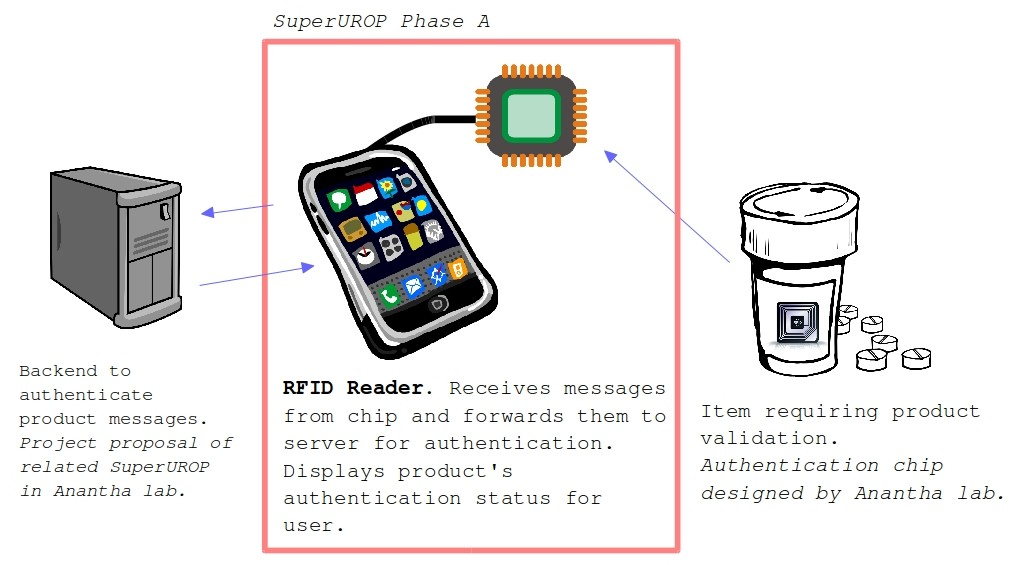
\includegraphics[scale=0.3]{skoppula-picture-1.jpg}
\end{center}

\textbf{A Voice Authentication System with Homomorphic Encryption}

Homomorphic encryption is a method of encryption that allows computing over ciphertext; not surprisingly, this form of encryption could be highly applicable in situations where untrusted parties provide important computing services on personal data. Unfortunately, most implementations of homomorphic-based computations have runtime disproportional to size of the input. Consequently, it makes sense to implement a homomorphic system in an application specific circuit, which may allow us to increase data throughput while still using minimal power.

For our computing application, we aim to prototype a service that authenticates users based on a voice sample. Specifically, this project aims to develop a system by which a homomorphically encrypted voice model is compared with input voice samples to determine which samples match the protected model.

The goal of this SuperUROP is to co-develop hardware-optimized algorithms necessary for voice recognition by way of homomorphic encryption of the models involved. After the related project confirms the feasibility of our algorithms in software models, this project plants to develop a hardware sketch in Bluespec Verilog that performs developed voice recognition algorithm. After simulated hardware testing, we aim to fabricate the designed chips to securely carry out voice recognition.

\begin{center}
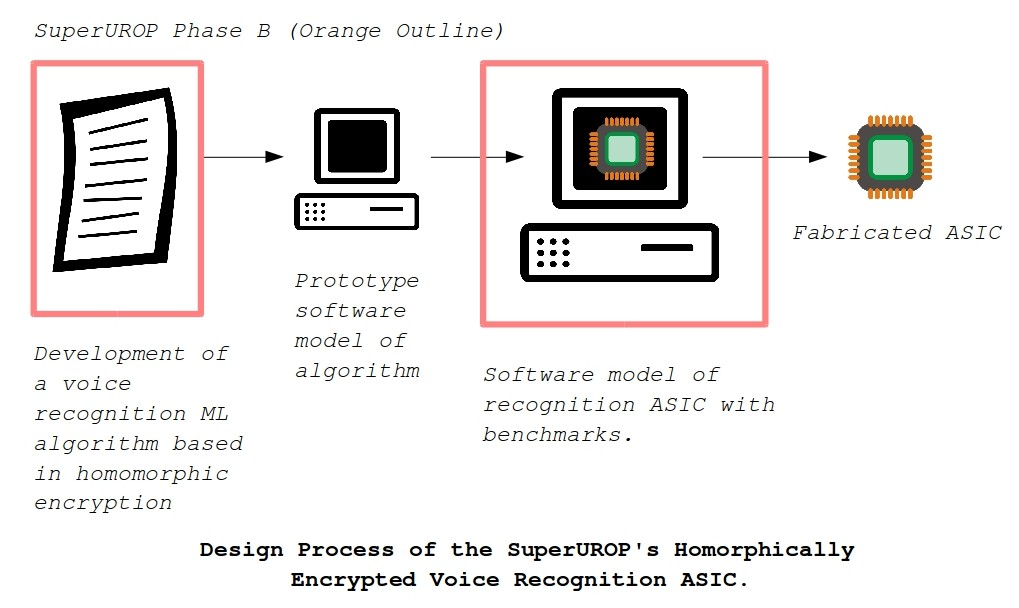
\includegraphics[scale=0.3]{skoppula-picture-2.jpg}
\end{center}

\end{document}

